\documentclass[11pt,a4paper]{article}
\usepackage[margin=2cm]{geometry}
\usepackage{amsmath,amssymb,amsthm}
\usepackage{tikz}
\usepackage{enumitem}
\usepackage[hidelinks]{hyperref}
\usepackage{titlesec}
\usepackage{xcolor}

\definecolor{accent}{HTML}{1F4E79}
\titleformat{\section}{\large\bfseries\color{accent}}{\thesection.}{0.5em}{}
\titlespacing*{\section}{0pt}{1.2em}{0.4em}
\setlist{itemsep=2pt,topsep=4pt}
\setlength{\parindent}{0pt}
\setlength{\parskip}{4pt}
\hypersetup{pdftitle={Parallelogram shaded triangle},pdfauthor={Krishnan}}

\newtheorem*{theorem}{Theorem}

\begin{document}

{\LARGE\bfseries\color{accent} Parallelogram shaded triangle}\par
\vspace{2pt}
{\small Kind: Problem \quad Date: 13-11-2026}
\vspace{6pt}\hrule\vspace{6pt}

\section{The problem}
\begin{minipage}[c]{0.55\linewidth}
$ABCD$ is a parallelogram with $AD = 5$. The point $P$ lies on $BC$ with $PC = 1$.
The diagonal $AC$ meets $DP$ at $X$. Find the fraction
\[
\frac{\text{area of } \triangle ADX}{\text{area of parallelogram } ABCD}.
\]
\textbf{What it asks:}
\begin{enumerate}
  \item The shaded triangle has vertices $A$, $D$ and $X = AC \cap DP$.
  \item Write $[F]$ for the area of a figure $F$. We need $[ADX] : [ABCD]$.
\end{enumerate}
\end{minipage}\hfill
\begin{minipage}[c]{0.42\linewidth}
\centering
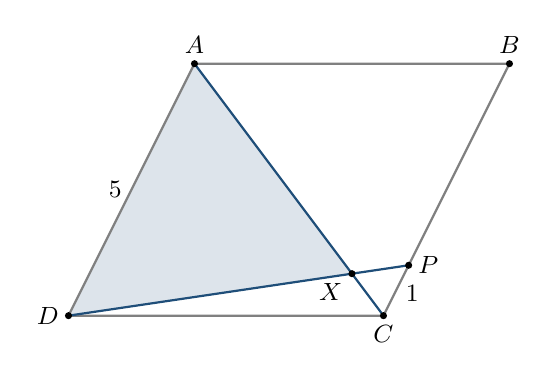
\begin{tikzpicture}[scale=0.8]
  \coordinate (D) at (0,0);   \coordinate (C) at (5,0);
  \coordinate (A) at (2,4);   \coordinate (B) at (7,4);
  \coordinate (P) at (5.4,0.8); \coordinate (X) at (4.5,0.6667);
  \fill[accent!15] (A) -- (D) -- (X) -- cycle;
  \draw[gray,thick] (A) -- (B) -- (C) -- (D) -- cycle;
  \draw[accent,thick] (A) -- (C);
  \draw[accent,thick] (D) -- (P);
  \node[left] at (1,2) {\small $5$};
  \node[right] at (5.2,0.35) {\small $1$};
  \foreach \p/\n/\pos in {A/A/above,B/B/above,C/C/below,D/D/left,P/P/right,X/X/below left}
    { \fill (\p) circle (1.6pt); \node[\pos] at (\p) {\small $\n$}; }
\end{tikzpicture}
\end{minipage}

\section{The idea in one line}
$AD \parallel CP$ makes $\triangle XAD \sim \triangle XCP$ with scale factor $5$, so $X$
divides $AC$ in the ratio $5:1$; then $[ADX] = \tfrac56[ADC] = \tfrac56\cdot\tfrac12[ABCD]$.

\section{Worked solution}
\begin{enumerate}
  \item \textbf{The diagonal halves the parallelogram.}
        In $\triangle ADC$ and $\triangle CBA$: $AD = CB$, $DC = BA$ (opposite sides of a
        parallelogram) and $AC$ is common. So $\triangle ADC \cong \triangle CBA$ (SSS), and
        \[ [ADC] = \tfrac12\,[ABCD]. \]
  \item \textbf{Two similar triangles.}
        $AD \parallel BC$ and $P$ lies on $BC$, so $AD \parallel CP$. In $\triangle XAD$ and
        $\triangle XCP$:
        \begin{itemize}
          \item $\angle AXD = \angle CXP$ \hfill (vertically opposite angles)
          \item $\angle XAD = \angle XCP$ \hfill (alternate angles, $AD \parallel CP$, transversal $AC$)
        \end{itemize}
        So $\triangle XAD \sim \triangle XCP$ (AA), with $A \leftrightarrow C$,
        $D \leftrightarrow P$, $X \leftrightarrow X$.
  \item \textbf{$X$ divides $AC$ in the ratio $5:1$.}
        Corresponding sides are in the same ratio:
        \[
          \frac{XA}{XC} = \frac{AD}{CP} = \frac{5}{1}
          \quad\Longrightarrow\quad AX = \tfrac56\,AC .
        \]
  \item \textbf{Same height, so areas are in the ratio of the bases.}
        $\triangle ADX$ and $\triangle ADC$ have the common vertex $D$ and bases $AX$ and $AC$
        on the same line. So they have the same height $h$ (the distance from $D$ to $AC$):
        \[
          \frac{[ADX]}{[ADC]} = \frac{\tfrac12\cdot AX\cdot h}{\tfrac12\cdot AC\cdot h}
          = \frac{AX}{AC} = \frac56 .
        \]
  \item \textbf{Combine.}
        \[
          [ADX] = \frac56\,[ADC] = \frac56\cdot\frac12\,[ABCD] = \frac{5}{12}\,[ABCD].
        \]
\end{enumerate}
\textbf{Answer.} The shaded triangle is $\boxed{\tfrac{5}{12}}$ of the parallelogram.

\section{Questions colleagues may ask}
\begin{enumerate}
  \item \textbf{Q. Is $BP = 4$ used anywhere?}
        No. Only $AD = 5$ and $CP = 1$ enter the solution. $BC = AD = 5$ only confirms that
        $P$ lies between $B$ and $C$.
  \item \textbf{Q. Does the answer depend on the shape of the parallelogram?}
        No. Every step uses only parallel lines and ratios along one line, so any
        parallelogram with $CP = \tfrac15 BC$ gives $\tfrac{5}{12}$. In general, if
        $CP = \tfrac1k BC$, then $AX : XC = k : 1$ and
        $[ADX] = \tfrac{k}{2(k+1)}\,[ABCD]$; for $k = 5$ this is $\tfrac{5}{12}$.
\end{enumerate}

\end{document}
